% Created 2015-04-05 sø 22:05
\documentclass[colorlinks=true,linkcolor=blue]{article}
\usepackage[utf8]{inputenc}
\usepackage[T1]{fontenc}
\usepackage{fixltx2e}
\usepackage{graphicx}
\usepackage{longtable}
\usepackage{float}
\usepackage{wrapfig}
\usepackage{rotating}
\usepackage[normalem]{ulem}
\usepackage{amsmath}
\usepackage{textcomp}
\usepackage{marvosym}
\usepackage{wasysym}
\usepackage{amssymb}
\usepackage{hyperref}
\tolerance=1000
\usepackage[top=1in,bottom=1in,left=1.2in,right=1.2in]{geometry}
\usepackage{pgf}
\usepackage{tikz}
\usetikzlibrary{arrows,automata}
\author{Sander Jespersen, Mathias Melgaard Andersen, Anders Roland Nielsen, \\ Andreas Berre Eriksen, Kent Munthe Caspersen \& Mikkel Alexander Madsen}
\date{\today}
\title{aMI Handin assignments}
\hypersetup{
  pdfkeywords={},
  pdfsubject={},
  pdfcreator={Emacs 24.3.1 (Org mode 8.2.10)}}
\begin{document}

\maketitle

\section{Water tank}
\label{sec-1}
\subsection{Baysian network}
\label{sec-1-1}
\begin{figure}[!htb]
  \centering
  \caption{Water tank model}
  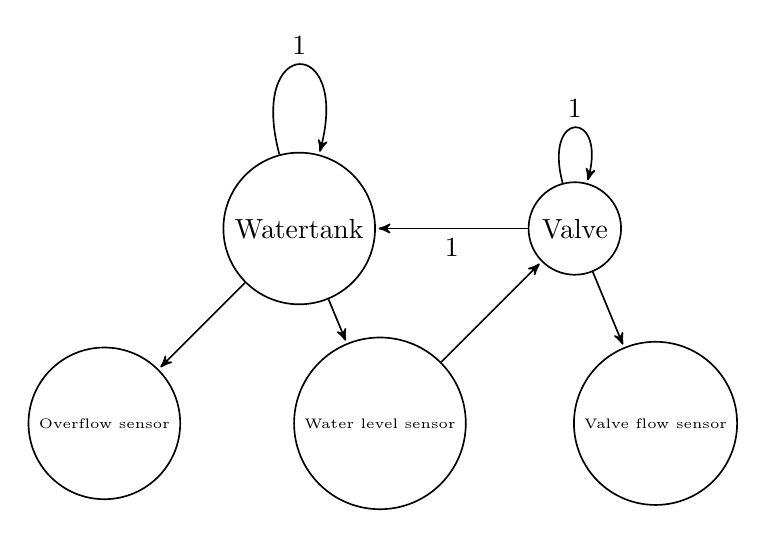
\begin{tikzpicture}[->,>=stealth',shorten >=1pt,auto,node distance=3.5cm, semithick]
    \tikzstyle{every state}=[draw]

    \node[state] (A)              {Watertank};
    \node[state] (B) [right of=A] {Valve};
    \node[state] (C) [below left of=A] {\tiny{Overflow sensor}};
    \node[state] (D) [right of=C] {\tiny{Water level sensor}};
    \node[state] (E) [right of=D] {\tiny{Valve flow sensor}};

    \path (A) edge node {} (C)
              edge node {} (D)
              edge [loop above] node {1} (A)
          (B) edge node {1} (A)
              edge node {} (E)
              edge [loop above] node {1} (B)
          (D) edge node {} (B);

  \end{tikzpicture}
  \label{fig:A1}
\end{figure}

\subsection{Suitable conditional probability distribution}
\label{sec-1-2}
Hvis ventil er åben fanger den stortset altid der er flow, hvis den er lukket laver den oftere fejl.

\begin{itemize}
\item Water tank:
\end{itemize}
\begin{center}
\begin{tabular}{l|rrrrrrrrrr|}
 & 0 & 1 & 2 & 3 & 4 & 5 & 6 & 7 & 8 & 9\\
\hline
L0 & 0.02 & 0.95 & 0.95 & 0.96 & 0.96 & 0.99 & 0.99 & 0.99 & 0.99 & 0.99\\
L10 & 0 & 0.98 & 0 & 0.0038 & 0 & 0.033 & 0.0016 & $7.97e^{-5}$ & $3.94e^{-6}$ & $1.95e^{-7}$\\
L20 & 0 & 0 & 0.049 & 0 & 0.033 & 0.0016 & $7.97e^{-5}$ & $3.94e^{-6}$ & $1.95e^{-7}$ & $9.66e^{-9}$\\
L30 & 0 & 0 & 0 & 0.045 & 0 & 0 & 0 & 0 & 0 & 0\\
Overflow & 0 & 0 & 0 & 0 & 0.012 & 0.011 & 0.011 & 0.011 & 0.011 & 0.011\\
\end{tabular}
\end{center}


\begin{center}
\begin{tabular}{l|rrrrr|}
 & 10 & 11 & 12 & 13 & 14\\
\hline
L0 & 0.99 & 0.99 & 0.99 & 0.99 & 0.99\\
L10 & $9.66e^{-9}$ & $4.78e^{-10}$ & $2.37e^{-11}$ & \$ 1.17e$^{\text{-12}}$\$ & \$ 5.80e$^{\text{-14}}$\$\\
L20 & $4.78e^{-10}$ & $2.37e^{-11}$ & \$ 1.17e$^{\text{-12}}$\$ & \$ 5.80e$^{\text{-14}}$\$ & \$ 2.87e$^{\text{-15}}$\$\\
L30 & 0 & 0 & 0 & 0 & 0\\
Overflow & 0.011 & 0.011 & 0.011 & 0.011 & 0.011\\
\end{tabular}
\end{center}

\begin{itemize}
\item Valve:
\end{itemize}
\begin{center}
\begin{tabular}{l|rrrrrrrrr|}
 & 0 & 1 & 2 & 3 & 4 & 5 & 6 & 7 & 8\\
\hline
Open & 0.02 & 0.95 & 0.96 & 0.97 & 0.96 & 0.95 & 0.94 & 0.93 & 0.92\\
Closed & 0.98 & 0.039 & 0.035 & 0.0017 & 8.47e$^{\text{-5}}$ & 4.19e$^{\text{-6}}$ & 2.076e$^{\text{-7}}$ & 1.028e$^{\text{-8}}$ & 5.087e$^{\text{-10}}$\\
Open Broken & 0 & 0.0002 & 0.0097 & 0.019 & 0.029 & 0.038 & 0.048 & 0.057 & 0.067\\
Closed Broken & 0 & 0.0098 & 0.01 & 0.011 & 0.011 & 0.011 & 0.011 & 0.011 & 0.011\\
\end{tabular}
\end{center}

\begin{center}
\begin{tabular}{l|rrrrrr|}
 & 9 & 10 & 11 & 12 & 13 & 14\\
\hline
Open & 0.91 & 0.90 & 0.9 & 0.89 & 0.88 & 0.87\\
Closed & $2.52e^{-11}$ & 1.25e$^{\text{-12}}$ & 6.17e$^{\text{-14}}$ & 3.054e$^{\text{-15}}$ & 1.51e$^{\text{-16}}$ & 7.48e$^{\text{-18}}$\\
Open Broken & 0.076 & 0.085 & 0.094 & 0.1 & 0.11 & 0.12\\
Closed Broken & 0.011 & 0.011 & 0.011 & 0.01 & 0.01 & 0.011\\
\end{tabular}
\end{center}

\begin{itemize}
\item Overflow sensor:
\end{itemize}
\begin{center}
\begin{tabular}{l|rrrrrrrrrrrrrrr|}
 & 0 & 1 & 2 & 3 & 4 & 5 & 6 & 7 & 8 & 9 & 10 & 11 & 12 & 13 & 14\\
\hline
water & 0.05 & 0.05 & 0.05 & 0.05 & 0.06 & 0.06 & 0.06 & 0.06 & 0.06 & 0.06 & 0.06 & 0.06 & 0.06 & 0.06 & 0.06\\
nowater & 0.95 & 0.95 & 0.95 & 0.95 & 0.94 & 0.94 & 0.94 & 0.94 & 0.94 & 0.94 & 0.94 & 0.94 & 0.94 & 0.94 & 0.94\\
\end{tabular}
\end{center}

\begin{itemize}
\item Water level sensor:
\end{itemize}
\begin{center}
\begin{tabular}{l|rrrrrrrrrrrrrrr|}
 & 0 & 1 & 2 & 3 & 4 & 5 & 6 & 7 & 8 & 9 & 10 & 11 & 12 & 13 & 14\\
\hline
L0 & 0.90 & 0.06 & 0.86 & 0.86 & 0.86 & 0.86 & 0.89 & 0.89 & 0.89 & 0.90 & 0.89 & 0.89 & 0.89 & 0.89 & 0.89\\
L10 & 0.05 & 0.88 & 0.05 & 0.05 & 0.05 & 0.08 & 0.05 & 0.05 & 0.05 & 0.05 & 0.05 & 0.05 & 0.05 & 0.05 & 0.05\\
L20 & 0.03 & 0.04 & 0.07 & 0.03 & 0.06 & 0.03 & 0.03 & 0.03 & 0.03 & 0.03 & 0.03 & 0.03 & 0.03 & 0.03 & 0.03\\
L30 & 0.02 & 0.02 & 0.02 & 0.06 & 0.03 & 0.03 & 0.03 & 0.03 & 0.03 & 0.03 & 0.03 & 0.03 & 0.03 & 0.03 & 0.03\\
\end{tabular}
\end{center}


\begin{itemize}
\item Valve flow sensor:
\end{itemize}
\begin{center}
\begin{tabular}{l|rrrrrrrrrrrrrrr|}
 & 0 & 1 & 2 & 3 & 4 & 5 & 6 & 7 & 8 & 9 & 10 & 11 & 12 & 13 & 14\\
\hline
Flow & 0.07 & 0.94 & 0.95 & 0.98 & 0.98 & 0.98 & 0.98 & 0.98 & 0.98 & 0.98 & 0.98 & 0.98 & 0.98 & 0.98 & 0.98\\
No flow & 0.93 & 0.06 & 0.05 & 0.02 & 0.02 & 0.02 & 0.02 & 0.02 & 0.02 & 0.02 & 0.02 & 0.02 & 0.02 & 0.02 & 0.02\\
\end{tabular}
\end{center}

\subsection{Simulation}
\label{sec-1-3}
We assume that only the controller has access to the water level sensor, and thus we can not manually read the water level through the sensor.

\section{Matlab}
\label{sec-2}
\subsection{Forward-backward algorithm}
\label{sec-2-1}
The changes we did to the given code was as follows:
\begin{itemize}
\item In the HMM class we added a backwardMessages
\item We initialised it to NaN when a HMM object was created
\end{itemize}
\begin{verbatim}
backwardMessages;

function obj = HMM(priorModel, transModel, sensorModel)
  ...
  obj.backwardMessages = NaN;
end
\end{verbatim}

The code below is our implementation of the backward part of the algorithm. The linebreak in the code is not present in the actual code but was done to fit on the page.

\begin{verbatim}
function obj = backward(obj, data)
  totalTime = length(data);

  obj.backwardMessages=zeros(obj.noHidden,totalTime+1);           

  obj.backwardMessages(:,totalTime+1) = 1;
    for t=totalTime:-1:1,
      obj.backwardMessages(:,t) 
      = obj.transModel*obj.sensorModel{data(t)}*obj.backwardMessages(:,t+1);
      obj.backwardMessages(:,t) 
      = obj.backwardMessages(:,t)./sum(obj.backwardMessages(:,t));
    end
end
\end{verbatim}

The result of running the our function on the given demo that forward was run on gives the following result:

\begin{center}
\begin{tabular}{rrrrrr}
0.6469 & 0.5923 & 0.3763 & 0.6533 & 0.6273 & 1.0000\\
0.3531 & 0.4077 & 0.6237 & 0.3467 & 0.3727 & 1.0000\\
\end{tabular}
\end{center}

\subsection{HMM for exercise 1}
\label{sec-2-2}
\begin{verbatim}
Trans = [ 0.8, 0.2; 
	  0.2, 0.8 ];
Prio = [ 0.6, 0.4 ]';
Sens = [ 0.02, 0.21; 
	 0.18, 0.49; 
	 0.08, 0.09; 
	 0.72, 0.21 ]';

% 1=yes+red, 2=yes+not red,  3=no+red, 4=no+not red
Dat = [ 4, 2, 1 ];

newhmm = HMM(Prio, Trans, Sens);
newhmm = newhmm.forward(Dat);
newhmm = newhmm.backward(Dat);

disp('Forward:');
disp(newhmm.forwardMessages);
disp('Backward:');
disp(newhmm.backwardMessages);
\end{verbatim}

\subsection{Implementation of HMM}
\label{sec-2-3}
\begin{itemize}
\item Forward:
\begin{center}
\begin{tabular}{rrr}
0.8372 & 0.4643 & 0.0804\\
0.1628 & 0.5357 & 0.9196\\
\end{tabular}
\end{center}

\item Backward:
\end{itemize}
\begin{center}
\begin{tabular}{rrrr}
0.5325 & 0.2661 & 0.2522 & 1.0000\\
0.4675 & 0.7339 & 0.7478 & 1.0000\\
\end{tabular}
\end{center}
\section{Exercise 3}
\label{sec-3}
\subsection{Umbrella}
\label{sec-3-1}
\begin{itemize}
\item By calculating the likelihood of the models correctness and the one with the highest likelihood is the most reliable model:
\begin{itemize}
\item 0.7 $\cdot$ 0.7 $\cdot$ 0.7 $\cdot$ 0.3 $\cdot$ 0.7 $\cdot$ 0.7 $\cdot$ 0.3 $\cdot$ 0.3 $\cdot$ 0.7 = 0.003176523
\item 0.6 $\cdot$ 0.6 $\cdot$ 0.6 $\cdot$ 0.4 $\cdot$ 0.8 $\cdot$ 0.8 $\cdot$ 0.2 $\cdot$ 0.4 $\cdot$ 0.8 = 0.003538944
\end{itemize}
\item Matlab
\end{itemize}
\begin{verbatim}
function p = SSP(obj, sequence)
  p = 1;
  for t=2:length(sequence),
    transition = obj.transModel(sequence(t-1),sequence(t));
    p = p * transition;                
  end
end
\end{verbatim}
\begin{itemize}
\item MATLAB gave us the same results as the manual calculations of the likelihood.
\end{itemize}


\subsection{Water tank}
\label{sec-3-2}
\begin{itemize}
\item Kalman Filter
\end{itemize}
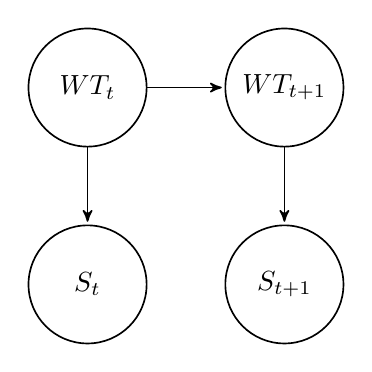
\begin{tikzpicture}[->,>=stealth',shorten >=1pt,auto,node distance=2.5cm, semithick]

\node[state, minimum size=1.5cm] (B) {$WT_t$};
\node[state, minimum size=1.5cm] (C) [below of = B] {$S_t$};
\node[state, minimum size=1.5cm] (D) [right of = B] {$WT_{t+1}$};
\node[state, minimum size=1.5cm] (E) [right of = C] {$S_{t+1}$};

\path (B) edge (D)
      (B) edge (C)
      (D) edge (E);

\end{tikzpicture}
\begin{enumerate}
\item $WT_{t+1} = \mathcal{N}(WT_t,1)$
\item $S_t = \mathcal{N}(WT_t,1.5)$
\end{enumerate}

\begin{itemize}
\item Filtered estimates:
\end{itemize}
\begin{align*}
\mu_{t+1} &= \frac{(1+1) \cdot 44 + 1.5 \cdot 50}{1 + 1 + 1.5} = 46.57 & \sigma^2_{t+1} &= \frac{(1+1) \cdot 1.5}{1 + 1 + 1.5} = 0.857 \\
\mu_{t+2} &= \frac{(0.857+1) \cdot 56 + 1.5 \cdot 46.57}{0.857 + 1 + 1.5} = 51.786 & \sigma^2_{t+2} &= \frac{(0.857+1) \cdot 1.5}{0.857 + 1 + 1.5} = 0.0.83\\
\mu_{t+3} &= \frac{(0.83+1) \cdot 49 + 1.5 \cdot 51.786}{0.83 + 1 + 1.5} = 50.25 & \sigma^2_{t+3} &= \frac{(0.83+1) \cdot 1.5}{0.83 + 1 + 1.5} = 0.82 \\
\mu_{t+4} &= \frac{(0.82+1) \cdot 51 + 1.5 \cdot 50.25}{0.82 + 1 + 1.5} = 50.66 & \sigma^2_{t+4} &= \frac{(0.82+1) \cdot 1.5}{0.82 + 1 + 1.5} = 0.82
\end{align*}

\begin{align*}
x &= \frac{(x+1) \cdot 1.5}{x+1+1.5}\\
x &= \frac{(x+1) \cdot 1.5}{x+2.5}\\
x(x+2.5) &= 1.5x + 1.5\\
x^2 + 2.5x &= 1.5x + 1.5\\
x^2+ x - 1.5 &= 0
\end{align*}

d = 1$^{\text{2}}$ - 4 $\cdot$ 1 $\cdot$ -1.5 = 7

$x = \frac{-1 \pm \sqrt{7}}{2 \cdot 1} = 
\begin{cases} x = \frac{-1 + \sqrt{7}}{2 \cdot 1} = 0.823\\
              x = \frac{-1 - \sqrt{7}}{2 \cdot 1} = -1.823
\end{cases}$


\section{Exercise 4}
\label{sec-4}
\subsection{Incomplete observations}
\label{sec-4-1}
\begin{itemize}
\item The starting values:
\end{itemize}

\begin{flalign*}
  P(R_0) &= (0.5, 0.5)\\
  P(R_t \mid R_{t-1} = t) &= (0.7, 0.3)\\
  P(R_t \mid R_{t-1} = f) &= (0.3, 0,7)\\
  P(U_t \mid R_t = t) &= (0.9, 0.1)\\
  P(U_t \mid R_t = f) &= (0.2, 0.8)
\end{flalign*}

\begin{align*}
S_1 &= (U, \neg U, U)\\
S_2 &= (U, \neg U, \neg U)
\end{align*}

\begin{itemize}
\item Forward og backward hvor C er normaliseringskonstant:
\end{itemize}
\begin{align*}
P(R_0 = i\mid S) &= \alpha_i(i)\beta_i(i) \cdot C\\
P(R_0 \mid S_1) &= (0.4827, 0.0745) \cdot C\\
P(R_0 \mid S_2) &= (0.4692, 0.0775) \cdot C\\
P(R_0 \mid S) &= (0.9519, 0.1520) \cdot  C = (0.8623, 0.1377)
\end{align*}

Næste skridt
\begin{align*}
P(R_{t-1}, R_t \mid S) &= \alpha(t-1) P(R_t \mid R_{t-1}) P(U_T \mid R_t) \beta(t)\\
P(R_1, R_2 \mid S_1) &= \alpha(1)P(R_2 \mid R_1)P(U_2 \mid R_2)\beta(2)
\end{align*}

\begin{align*}
forward_0 \cdot backward_1 \cdot Trans \cdot Sensor &= x\\
0.8182 \cdot 0.3695 \cdot 0.7 \cdot 0.1 &= 0.0212 \\
0.8182 \cdot 0.6305 \cdot 0.3 \cdot 0.8 &= 0.1256 \\
0.1818 \cdot 0.3695 \cdot 0.3 \cdot 0.1 &= 0.0020 \\
0.1818 \cdot 0.6395 \cdot 0.7 \cdot 0.8 &= 0.0642 
\end{align*}

\begin{align*}
forward_1 \cdot backward_2 \cdot Trans \cdot Sensor &= x\\
0.1738 \cdot 0.6273 \cdot 0.7 \cdot 0.9 &= 0.0687 \\
0.1738 \cdot 0.3737 \cdot 0.3 \cdot 0.2 &= 0.0039 \\
0.8268 \cdot 0.6273 \cdot 0.3 \cdot 0.9 &= 0.1400 \\
0.8268 \cdot 0.3737 \cdot 0.7 \cdot 0.2 &= 0.0433 
\end{align*}

New trans model
\begin{align*}
P(R_t = T \mid R_{t-1} = T) &= 0.0212 + 0.0687 = 0.0899\\
P(R_t = F \mid R_{t-1} = T) &= 0.0687 + 0.0039 = 0.1295\\
P(R_t = T \mid R_{t-1} = F) &= 0.0020 + 0.1400 = 0.1420\\
P(R_t = F \mid R_{t-1} = F) &= 0.0642 + 0.0433 = 0.1075
\end{align*}
\begin{center}
\begin{tabular}{l|rr}
 & T & F\\
\hline
T & 0.0899 & 0.1295\\
F & 0.1420 & 0.1075\\
\end{tabular}
\end{center}

New Sensor model

Umbrella is true:
\begin{align*}
P(R_1 \mid S_{1_{top}}) &= 0.8182 \cdot 0.5900 = 0.4827\\
P(R_1 \mid S_{1_{bot}}) &= 0.1818 \cdot 0.4100 = 0.0745\\
P(R_3 \mid S_{1_{top}}) &= 0.7251 \cdot 0.6273 = 0.4549\\
P(R_3 \mid S_{1_{bot}}) &= 0.2749 \cdot 0.3727 = 0.2702\\
P(R_1 \mid S_{2_{top}}) &= 0.8182 \cdot 0.5735 = 0.4692\\
P(R_1 \mid S_{2_{bot}}) &= 0.1818 \cdot 0.4264 = 0.0775
\end{align*}

Summation of top and bottom respectively:
\begin{align*}
0.4827 + 0.4549 + 0.4692 &= 1.4068\\
0.0745 + 0.2702 + 0.0775 &= 0.4222
\end{align*}

Umbrella is false:
\begin{align*}
P(R_2 \mid S_{1_{top}}) &= 0.1738 \cdot 0.3695 = 0.0642\\
P(R_2 \mid S_{1_{bot}}) &= 0.8262 \cdot 0.6305 = 0.5209\\
P(R_2 \mid S_{2_{top}}) &= 0.1738 \cdot 0.3247 = 0.0564\\
P(R_2 \mid S_{2_{bot}}) &= 0.8262 \cdot 0.6753 = 0.5579\\
P(R_3 \mid S_{2_{top}}) &= 0.0683 \cdot 0.3444 = 0.0235\\
P(R_3 \mid S_{2_{bot}}) &= 0.9317 \cdot 0.6556 = 0.6108
\end{align*}

Summation of top and bottom respectively:
\begin{align*}
0.0642 + 0.0564 + 0.0235 &= 0.1441\\
0.5209 + 0.5579 + 0.6108 &= 1.6896
\end{align*}

Normalisation of table:
\begin{center}
\begin{tabular}{l|rr}
 & T & F\\
\hline
T & 0.9071 & 0.0929\\
F & 0.1999 & 0.8001\\
\end{tabular}
\end{center}
\section{Exercise 5}
\label{sec-5}
\subsection{Slide 19 example}
\label{sec-5-1}

The formula: $\gamma = 0.9$
\begin{align*}
U³(x,y) &= R(x,y) + \gamma \cdot max_{a \in \{left,right,up,down\} } \sum_{s'\in S} P(s' \mid a,s) U^2(s')\\
U³(2,1) &=
\begin{aligned}
  -0.1 + 0.9 \cdot max(0.7 &\cdot -0.63 + 0.1 \cdot -5.17 + 0.1 \cdot -0.19 + 0.1 \cdot -0.19,\\ 
  0.7 &\cdot -5.17 + 0.1 \cdot -0.63 + 0.1 \cdot -0.19 + 0.1 \cdot -0.19,\\ 
  0.7 &\cdot -0.19 + 0.1 \cdot -0.63 + 0.1 \cdot -5.17 + 0.1 \cdot -0.19,\\ 
  0.7 &\cdot -0.19 + 0.1 \cdot -0.63 + 0.1 \cdot -5.17 + 0.1 \cdot -0.19)
\end{aligned}
\\
U³(2,1) &= -0.1 + 0.9 \cdot max(-0.996,-3.72,-0.732,-0.732)\\
U³(2,1) &= -0.7588
\end{align*}
\begin{center}
\begin{tabular}{r|r|r|r|}
 & 1 & 2 & 3\\
\hline
1 & 3.42 & 6.23 & 10\\
\hline
2 & -0.76 & -1.07 & 5.24\\
\hline
3 & -0.35 & -0.77 & 2.79\\
\hline
\end{tabular}
\end{center}

\subsection{Policy iteration}
\label{sec-5-2}
% Emacs 24.3.1 (Org mode 8.2.10)
\end{document}